% ========================================= TEMPLATE INFO ========================================
%
% Author:       P4ntomime
% Version:      1.0.1
% Last updated: 2026-01-24
% Brief:        A LaTeX template for summaries. See README.md for more information.
% 
% ================================================================================================
\documentclass[8pt, a4paper, twoside, landscape]{extarticle}
% Font size:    8pt
% Paper size:   A4
% style:        twoside (needed, so odd and even pages have different margins)
% orientation:  portrait. (use 'landscape' for landscape orientation)


% ========================================= DOCUMENT INFO =========================================
\def\title{Prog-Py}                   % title
\def\shorttitle{Prog-Py}         % short title (displayed as PDF title)
\def\dozent{Prof. Selina Rea Malacarne}                 % lecturer
\def\semester{FS2026}             % semester
\def\author{Mirko Ratti}                % author(s)
% \def\contributors{Contributors}     % contributor(s) (optional -> comment out if none)
\def\repo{https://github.com/P4ntomime/TeXFoSaTemplate} % repository link
\def\version{1.0.\today}            % version
\def\pagelimit{20}                   % page limit -> causes pages after limit to be red
\def\titleoption{ultra compact}     % options: ultra compact, compact, normal
\def\enableToC{false}                % enable/disable table of contents

% ================================= PACKAGES, SETUP AND COMMANDS ==================================
\input{preamble.tex}


% =========================================== DOCUMENT ============================================
\begin{document}
    \begin{layout}
        \section{Python Overview}
\begin{itemize}
    \item \textbf{Origins:} Developed by Guido van Rossum with a focus on simplicity and power.
    \item \textbf{Standard Library:} Known for the "batteries included" philosophy, meaning it comes with an extensive built-in library.
    \item \textbf{Ecosystem:} For engineering tasks, Python replaces Matlab toolboxes with specialized packages like \textbf{NumPy} (numerical data), \textbf{pandas} (data processing), and \textbf{matplotlib} (visualization).
\end{itemize}

\section{Variables and Objects}
In Python, everything is an object. Variables are not containers but \textbf{references} (pointers) bound to objects.

\begin{minipage}{0.4\columnwidth}
    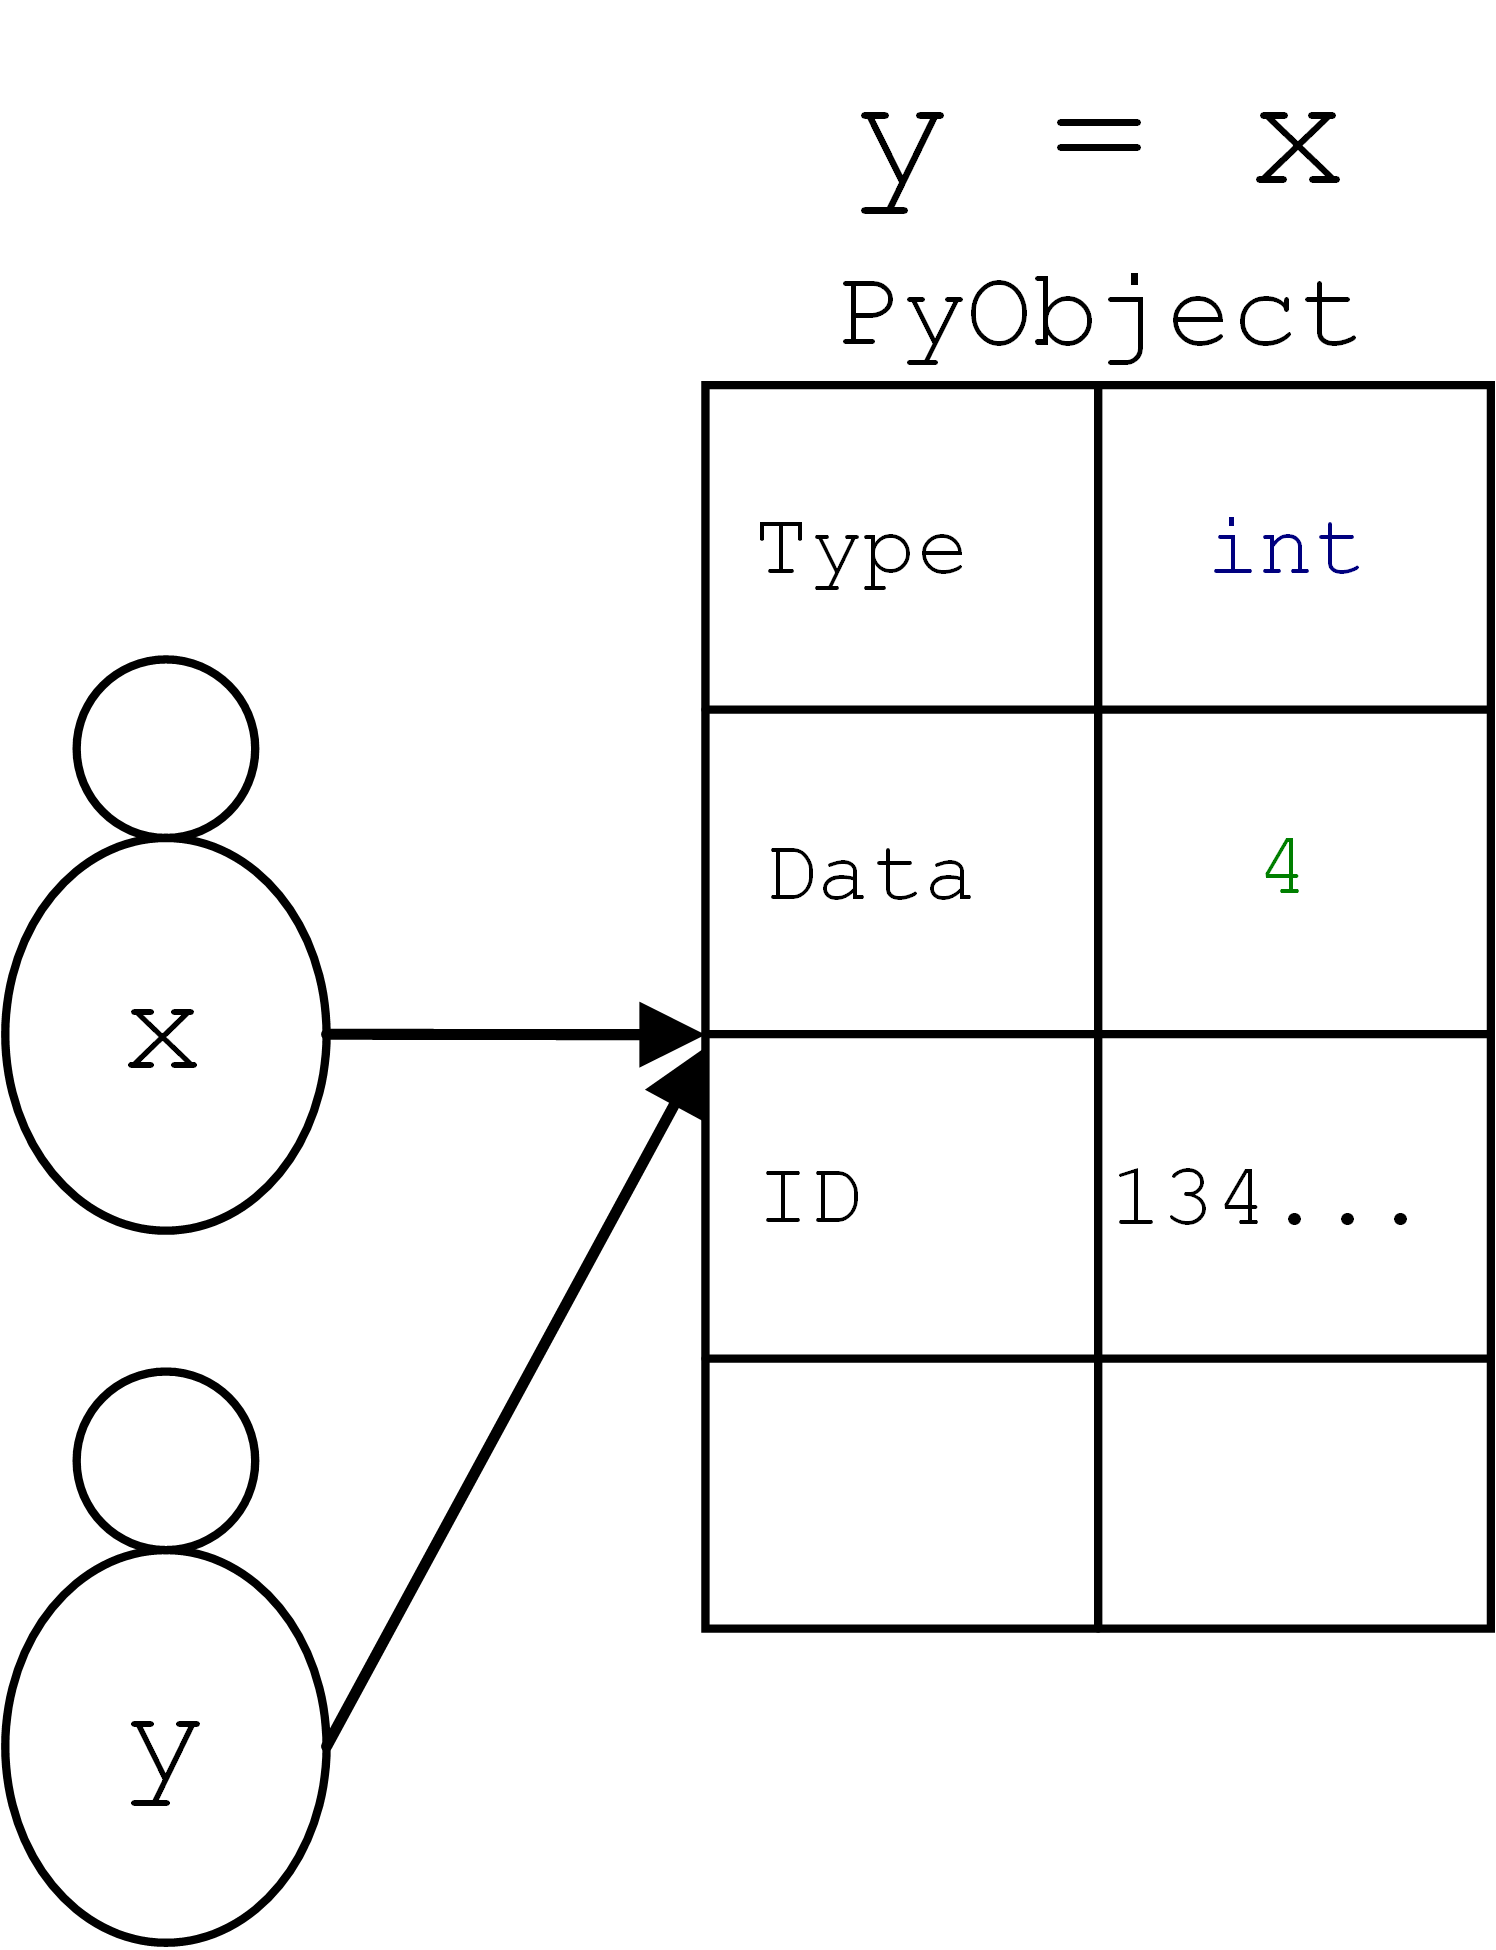
\includegraphics[width=\linewidth]{images/var_2.png}
\end{minipage}\hfil
\begin{minipage}{0.4\columnwidth}
    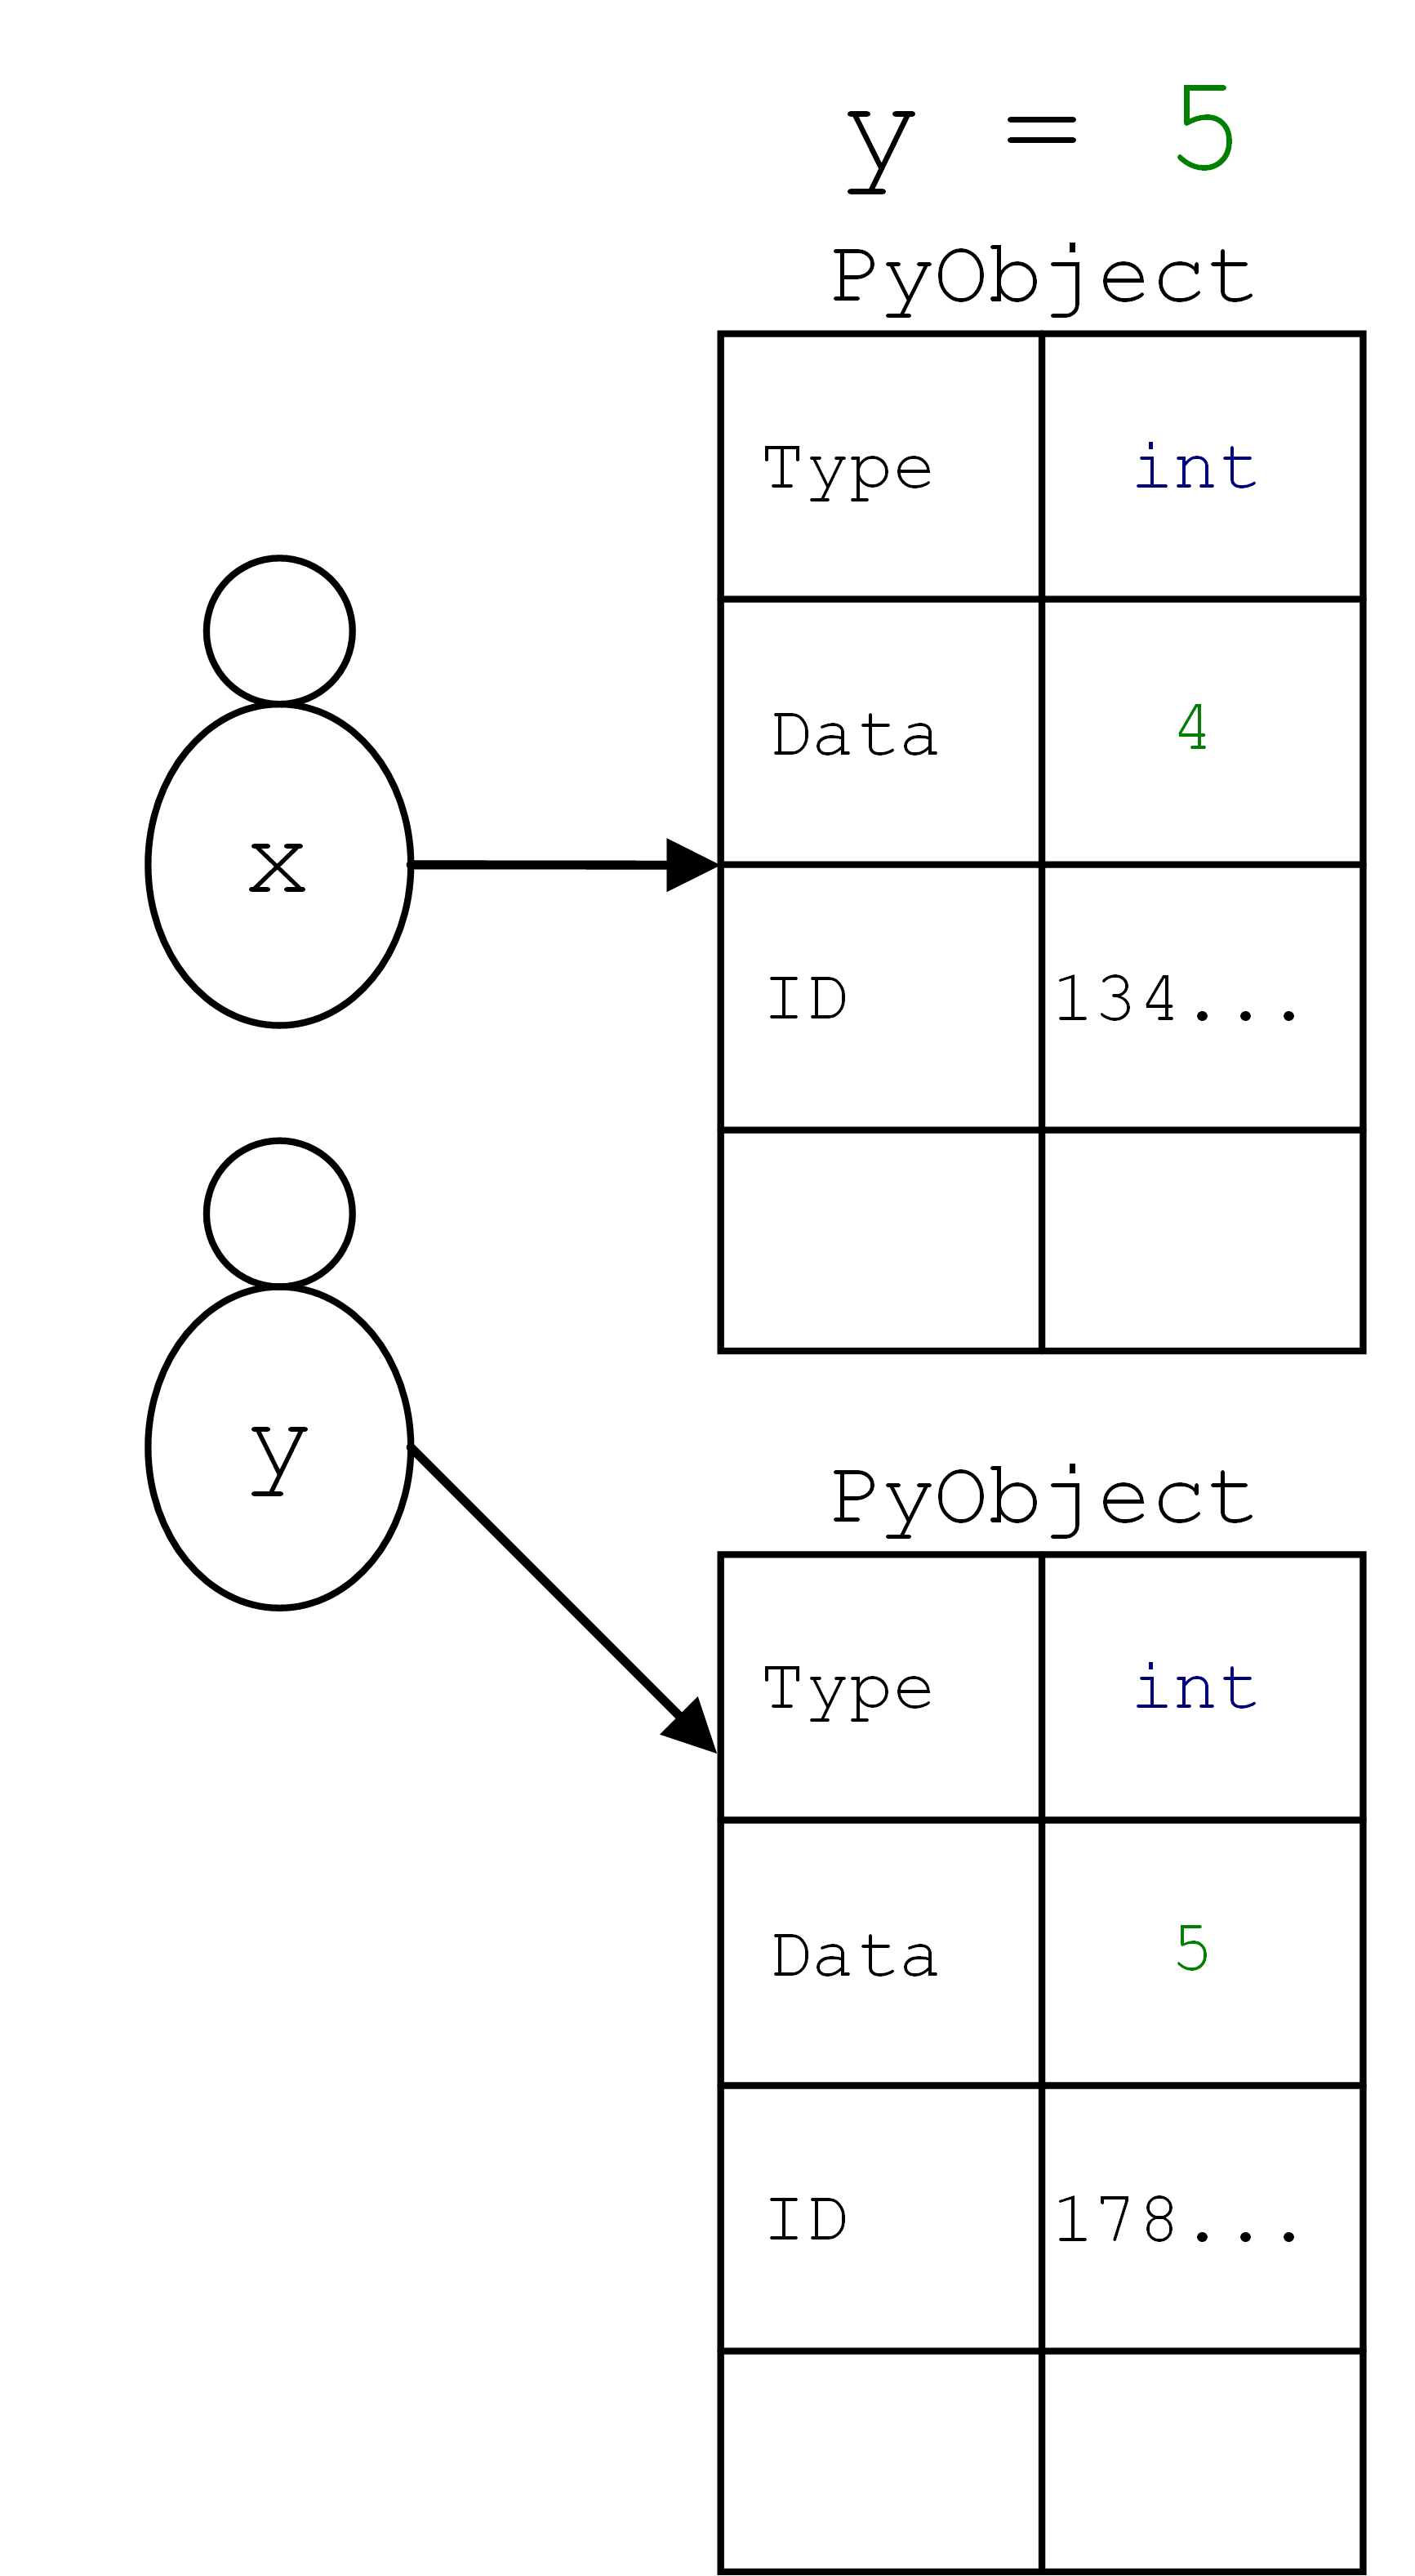
\includegraphics[width=\linewidth]{images/var_3.png}
\end{minipage}

\subsection{Built-in Data Types}
\begin{center}
    \begin{tabular}{llll}
        \toprule
        \textbf{Category} & \textbf{Data Type} & \textbf{Mutability} & \textbf{False Value} \\ \midrule
        \textbf{None} & \texttt{NoneType} & Immutable & \texttt{None} \\ \addlinespace
        \textbf{Numeric} & \texttt{int} & Immutable & \texttt{0} \\
        & \texttt{float} & Immutable & \texttt{0.0} \\
        & \texttt{bool} & Immutable & \texttt{False} \\
        & \texttt{complex} & Immutable & \texttt{0 + 0j} \\ \addlinespace
        \textbf{Sequence} & \texttt{str} & Immutable & \texttt{''} \\
        & \texttt{list} & Mutable & \texttt{[]} \\
        & \texttt{tuple} & Immutable & \texttt{()} \\
        & \texttt{bytes} & Immutable & \texttt{b''} \\
        & \texttt{bytearray} & Mutable & \texttt{bytearray(b'')} \\ \addlinespace
        \textbf{Sets} & \texttt{set} & Mutable & \texttt{set()} \\
        & \texttt{frozenset} & Immutable & \texttt{frozenset()} \\ \addlinespace
        \textbf{Associative} & \texttt{dict} & Mutable & \texttt{\{\}} \\ \bottomrule
    \end{tabular}
\end{center}

\subsection{Mutability}
\begin{itemize}
    \item \textbf{Immutable:} Objects that cannot be modified after creation (e.g., \texttt{int}, \texttt{float}, \texttt{str}, \texttt{tuple}). Changing the value of an immutable variable actually creates a new object in memory.
    \item \textbf{Mutable:} Objects that can be modified in-place (e.g., \texttt{list}, \texttt{set}, \texttt{dict}).
\end{itemize}\vspace{1em}
The memory address of an object, can be visuasalized using the \texttt{id()} function. 

It returns a unique integer for the given object.

\section{Namespaces and Scope}
A namespace is a system (implemented as a dictionary) that ensures all names in a program are unique and can be used without conflict.

\begin{itemize}
    \item \textbf{Built-in:} Contains all integrated symbols available in Python (e.g., \texttt{print()}).
    \item \textbf{Global:} Symbols defined at the top level of a module or script.
    \item \textbf{Local:} Created for specific scopes, such as within a function.
    \item \textbf{LEGB Rule:} Python searches for names from the inside out: \textbf{L}ocal $\rightarrow$ \textbf{G}lobal $\rightarrow$ \textbf{B}uilt-in.
\end{itemize}

Built-in symbols can be overwritten by the user, however, it is not recommended.

\section{Arithmetic and Magic Methods}
\begin{itemize}
    \item \textbf{Special Operators:} \texttt{//} (integer division), \texttt{\%} (modulo/remainder), and \texttt{**} (exponentiation).
    \item \textbf{Syntactic Sugar:} Operators are just a "friendly" way to call internal methods. For example, \texttt{x + y} is internally executed as \texttt{x.\_\_add\_\_(y)}.
\end{itemize}

\begin{center}
    \small
    \begin{tabular}{lll}
    \toprule
    \textbf{Operator} & \textbf{Dunder Method} & \textbf{Description} \\ \midrule
    \texttt{x + y} & \texttt{x.\_\_add\_\_(y)} & Sum \\
    \texttt{x - y} & \texttt{x.\_\_sub\_\_(y)} & Difference \\
    \texttt{x * y} & \texttt{x.\_\_mul\_\_(y)} & Product \\
    \texttt{x / y} & \texttt{x.\_\_truediv\_\_(y)} & Quotient \\
    \texttt{x // y} & \texttt{x.\_\_floordiv\_\_(y)} & Floored quotient$^1$ \\
    \texttt{x \% y} & \texttt{x.\_\_mod\_\_(y)} & Remainder (Modulo)$^1$ \\
    \texttt{x ** y} & \texttt{x.\_\_pow\_\_(y)} & Exponentiation ($x^y$) \\
    \texttt{abs(x)} & \texttt{x.\_\_abs\_\_()} & Absolute value \\
    \texttt{-x} & \texttt{x.\_\_neg\_\_()} & Negative sign \\ \midrule
    \multicolumn{3}{l}{\small $^1$ Operator not defined for the data type \texttt{complex}} \\ \bottomrule
    \end{tabular}
\end{center}

\subsection*{Code Example}
Ecco come Python interpreta gli operatori dietro le quinte:

\begin{lstlisting}[language=Python]
# Standard operator usage
result_a = 5 + 5

# Behind the scenes (Magic Method)
result_b = (5).__add__(5)

print(result_a == result_b) # Output: True
\end{lstlisting}
        \section{Conditional Branching}
\begin{itemize}
    \item \textbf{Basic Structures}: \texttt{if}, \texttt{elif}, and \texttt{else} execute code blocks based on conditions. Consistent indentation is required.
    \item \textbf{Match-case}: Introduced in Python 3.10 to recognize specific patterns and data structures.
\end{itemize}

\lstinputlisting[language=python]{code/conditions.py}

\subsection{Boolean Expressions and Operators}
\begin{itemize}
    \item \textbf{Walrus Operator (\texttt{:=})}: Assigns and returns a value within an expression.
    \item \textbf{Ternary Operator}: Compact syntax for simple single-line conditional assignments.
    \item \textbf{\texttt{==} vs \texttt{is}}:
    \begin{itemize}
        \item \texttt{==} checks value equality; 
        \item \texttt{is} checks object identity in memory (ideal for checking \texttt{None}).
    \end{itemize} 
    \item \textbf{\texttt{in} Operator}: Checks presence in objects implementing \texttt{\_\_contains\_\_()} (Only usable on iterable Objects: lists, strings, dicts).
\end{itemize}

\lstinputlisting[language=python]{code/boolean_expressions.py}

\subsection{Exception Handling}
\begin{itemize}
    \item \textbf{LBYL (Look Before You Leap)}: A defensive style where you explicitly check for conditions (\texttt{if os.path.exists}) before making a call. This can be prone to "race conditions" where the state changes between the check and the action.
    \item \textbf{EAFP (Easier to Ask Forgiveness than Permission)}: The 'Pythonic' approach. Assume the operation will succeed and wrap it in a \texttt{try/except} block. This is generally cleaner and more robust in multi-threaded environments.
    \item \textbf{Catching Exceptions}: Always catch specific exceptions (e.g., \texttt{FileNotFoundError}) rather than generic ones. Use the \texttt{as} keyword to inspect the exception object.
    \item \textbf{Flow Control}:
    \begin{itemize}
        \item \texttt{else}: Runs only if the \texttt{try} block succeeded without errors.
        \item \texttt{finally}: Always runs (e.g., for closing file handles), regardless of whether an exception was raised or caught.
    \end{itemize}
\end{itemize}

\lstinputlisting[language=python]{code/exceptions.py}

        \section{Iterations}
\subsection{Slicing}
\begin{itemize}
   \item Syntax: \texttt{part = x[start:end:step]}.
   \item Start is inclusive (default 0).
   \item End is exclusive (default end index).
   \item Step is optional (default 1). A negative step indicates reverse order.
\end{itemize}

\begin{lstlisting}[language=Python]
data = [0, 1, 2, 3, 4, 5.0, [1,2,3]]
part = data[::-1] # Reverse order
\end{lstlisting}

\subsection{For-loops}
\begin{itemize}
    \raggedright
    \item Internally calls \texttt{iter()} to return an iterator.
    \item Uses the \texttt{next(iterator)} method to get the next element until a \texttt{StopIteration} exception is raised.
\end{itemize}

\begin{lstlisting}[language=Python]
for value in iterable:
    expression1
\end{lstlisting}

\subsubsection{Loop-control statements}
\begin{itemize}
    \item \textbf{break}: Terminates a loop before completion.
    \item \textbf{continue}: Skips the remaining code in the loop for the current iteration.
    \item \textbf{else keyword}: Executed when the loop ends normally, meaning it has not encountered a \texttt{break} statement.
\end{itemize}

\subsubsection{Dictionaries}
\begin{lstlisting}[language=Python]
for key in data:                # Iterates keys
for value in data.values():     # Iterates values
for key, value in data.items(): # Iterates both keys and values
\end{lstlisting}

\subsubsection{Enumerate}
\begin{itemize}
    \item Used when a counter is needed while iterating through elements.
\end{itemize}

\begin{lstlisting}[language=Python]
for i, fruit in enumerate(fruits, start=10):
    print(i, fruit)
\end{lstlisting}

\subsubsection{Zip}
\begin{itemize}
    \item Iterates over multiple iterables at the same time.
    \item \textbf{Objects of different lengths}: The \texttt{zip()} function stops as soon as the shortest iterable is exhausted. Any remaining elements in the longer iterables are simply ignored.
\end{itemize}

\lstinputlisting[language=Python]{code/zip.py}

\subsection{Comprehensions}
\begin{itemize}
    \item \textbf{Base Syntax}: \texttt{[expression for item in iterable]}.
    \item \textbf{Nested for loops}: Evaluated from left to right.
    \item \textbf{Can also call functions}: Built-in functions, like \texttt{any()}, can be used.
    \item \textbf{\color{red}Conditional Syntax}: The position of the \texttt{if} statement completely changes its behavior. 
    \begin{itemize}
        \item \textbf{Filtering (Only \texttt{if})}: Must be placed at the \textbf{\color{orange}END}. It filters elements out of the iterable.
        \item \textbf{Modifying (\texttt{if/else})}: Must be placed at the \textbf{\color{orange}BEGINNING} (before the \texttt{for} loop). It changes the value of the element based on the condition but does not filter it out.
    \end{itemize}
\end{itemize}

\lstinputlisting[language=Python]{code/comprehensions.py}
        \section{Built in methods}
\subsection{Lists}

\textbf{Methods \texttt{sort()} and \texttt{sorted()}}
\begin{itemize}
    \item \texttt{sort()}: Modifies the list in-place. Allows a \texttt{reverse=True} parameter for descending order.
    \item \texttt{sorted()}: Returns a new sorted list and can be applied to all iterable objects.
    \item \textbf{The \texttt{key} Argument}: Allows specifying a custom sorting function. It accepts built-in functions (e.g., \texttt{str}) or anonymous \textit{lambda} functions for inline sorting criteria.
    \item \textbf{Algorithm Stability and Multiple Priorities}: Python utilizes 
    \textit{Timsort}, a stable sorting algorithm. Stability ensures that when two 
    elements share the same sorting key, they retain their original relative order. 
    To sort by multiple criteria, you can 'stack' consecutive sorts: you must apply 
    the \textit{least} priority sort first, and the \textit{main} priority filter last.
    Alternatively, you can use a single lambda function that returns a tuple 
    representing the hierarchy of priorities.
\end{itemize}

\lstinputlisting[language=Python]{code/sort_stacking.py}

\textbf{Indirect Sorting (Sorting Indices)}
In many algorithms, it is highly efficient to sort an array of indices rather than moving the actual data elements around. By leveraging a lambda function, we can sort a standard sequence of indices based on the values they point to in the original list.

\lstinputlisting[language=Python]{code/indirect_sorting.py}

\textbf{List Slicing}
Slicing extracts sub-sequences using the \texttt{x[start:end:step]} syntax. Besides extraction, slicing is extremely powerful for dynamically modifying lists: it allows replacing an entire area of elements or inserting multiple elements at a specific index simultaneously without overwriting existing data.

\begin{lstlisting}[language=Python]
data = ['a', 'b', 'c']
# Inserting multiple elements without replacing (at index 3)
data[3:3] = ['#', '$']   # Result: ['a', 'b', 'c', '#', '$']

# Replacing an entire area with new elements
data[1:3] = ['D', 'E']   # Result: ['a', 'D', 'E', '#', '$']
\end{lstlisting}

\subsection{Shallow and Deep Copy}
Variable assignment merely binds a name to an object; it does not create a copy.



\begin{itemize}
    \item \textbf{Shallow Copy}: Functions like \texttt{list()}, \texttt{dict()}, or \texttt{.copy()} create a new object only at the top level. Subordinate nested objects are only referenced, meaning modifications to mutable nested objects will affect both the original and the copy.
    \item \textbf{Deep Copy}: Creates a true, recursive copy of the object and all its subordinates.
\end{itemize}

\begin{lstlisting}[language=Python]
import copy
list1 = [[1, 2], [3, 4]]
list_shallow = list1.copy()
list_deep = copy.deepcopy(list1)
\end{lstlisting}

\subsection{Strings}

\textbf{Most Used Methods}
\begin{itemize}
    \item \textbf{Splitting and Cleaning}: \texttt{split(sep)} splits by a separator. \texttt{splitlines()} splits at line breaks. \texttt{strip()}, \texttt{lstrip()} remove leading/trailing characters.
    \item \textbf{Searching and Replacing}: \texttt{find(sub)}. \texttt{count(sub)}. \texttt{replace(old, new)}.
    \item \textbf{Casing}: \texttt{lower()}. \texttt{upper()}. \texttt{capitalize()}. \texttt{title()}.
    \item \textbf{Testing}: \texttt{isdigit()}. \texttt{isalpha()}. \texttt{isalnum()}. \texttt{islower()}. \texttt{isupper()}.
\end{itemize}

\textbf{\texttt{join()} and Generators}
The \texttt{join()} method combines all string elements of an iterable into a single string, using the calling string as a separator. It is highly efficient when combined with generator expressions.

\begin{lstlisting}[language=Python]
z = [(10, "Matthias"), (20, "Annabelle")]
# Joining elements using a generator expression
ranking = "\n".join(f"{name} ({points} Points)" for points, name in z)
\end{lstlisting}

\textbf{F-Strings Formatting}
Formatting logic follows the syntax: \texttt{\{<f\_expression> ["="] [!<conversion>] [:<format\_spec>]\}}. Self-documenting expressions can be created by adding an equal sign \texttt{=} after the variable name.

\vspace{1em}

\resizebox{\columnwidth}{!}{
\begin{tabular}{|l|l|l|l|}
\hline
\textbf{Parameter} & \textbf{Description} & \textbf{Example} & \textbf{Output} \\
\hline
\multicolumn{4}{|c|}{\textbf{Presentation Type (\texttt{<type>})}} \\
\hline
\texttt{b} & Binary Integer & \texttt{f'\{10:b\}'} & \texttt{'1010'} \\
\hline
\texttt{c} & Single Character & \texttt{f'\{65:c\}'} & \texttt{'A'} \\
\hline
\texttt{d} & Decimal Integer & \texttt{f'\{75:d\}'} & \texttt{'75'} \\
\hline
\texttt{e} or \texttt{E} & Exponential Form & \texttt{f'\{0.001:e\}'} & \texttt{'1.000000e-03'} \\
\hline
\texttt{f} or \texttt{F} & Float & \texttt{f'\{157:f\}'} & \texttt{'157.000000'} \\
\hline
\texttt{g} or \texttt{G} & Float or Exponential (based on size) & \texttt{f'\{15723823:G\}'} & \texttt{'1.57238E+07'} \\
\hline
\texttt{o} & Octal Integer & \texttt{f'\{16:o\}'} & \texttt{'20'} \\
\hline
\texttt{s} & String & \texttt{f'\{"Hallo":s\}'} & \texttt{'Hallo'} \\
\hline
\texttt{x} or \texttt{X} & Hexadecimal Integer & \texttt{f'\{10:X\}'} & \texttt{'A'} \\
\hline
\texttt{\%} & Percentage & \texttt{f'\{1:\%\}'} & \texttt{'100.000000\%'} \\
\hline
\multicolumn{4}{|c|}{\textbf{Alignment (\texttt{<align>})}} \\
\hline
\texttt{<} & Left-aligned & \texttt{f'\{12:<5\}'} & \texttt{'12   '} \\
\hline
\texttt{>} & Right-aligned & \texttt{f'\{12:>5\}'} & \texttt{'   12'} \\
\hline
\texttt{\^{}} & Centered & \texttt{f'\{12:\^{}5\}'} & \texttt{' 12  '} \\
\hline
\texttt{=} & Sign forced to the far left & \texttt{f'\{-12:=5\}'} & \texttt{'-  12'} \\
\hline
\multicolumn{4}{|c|}{\textbf{Fill Character (\texttt{<fill>})}} \\
\hline
\texttt{char} & Any character (used with align) & \texttt{f'\{12:\_>5\}'} & \texttt{'\_\_\_12'} \\
\hline
\multicolumn{4}{|c|}{\textbf{Sign (\texttt{<sign>})}} \\
\hline
\texttt{+} & Forces sign for positive/negative & \texttt{f'\{123:+\}'} & \texttt{'+123'} \\
\hline
\texttt{-} & Sign only for negative numbers & \texttt{f'\{-123:-\}'} & \texttt{'-123'} \\
\hline
\multicolumn{4}{|c|}{\textbf{Grouping (\texttt{<group>})}} \\
\hline
\texttt{,} or \texttt{\_} & Thousands separator & \texttt{f'\{1000:,\}'} & \texttt{'1,000'} \\
\hline
\multicolumn{4}{|c|}{\textbf{Width and Precision (\texttt{<width>.<precision>})}} \\
\hline
\texttt{width} & Minimum output width & \texttt{f'\{12:5\}'} & \texttt{'   12'} \\
\hline
\texttt{.precision} & Decimal places (for floats) & \texttt{f'\{3.14159:.2f\}'} & \texttt{'3.14'} \\
\hline
\end{tabular}}\vspace{1em}

With \# is possible to show the alternative output format (0xA10, 0b01101)

\subsection{Dictionaries}
\textbf{Most Used Methods}
\begin{itemize}
    \item \texttt{get(key, default)}: Returns the value for a key, or a default value (like \texttt{None}) if the key does not exist.
    \item \texttt{keys()}, \texttt{values()}, \texttt{items()}: Return views of the dictionary's keys, values, and key-value pairs, respectively.
    \item \texttt{setdefault(key, default)}: Returns the value of a key; if absent, it inserts the key with the specified default value.
    \item \texttt{pop(key)} and \texttt{popitem()}: Remove a specific key-value pair or the last added pair.
    \item \texttt{clear()}: Removes all key-value pairs.
\end{itemize}

\subsection{File Handling}
Files are handled using the \texttt{open()} function, which accepts a filename and a mode (e.g., \texttt{'r'} for reading, \texttt{'w'} for writing, \texttt{'a'} for appending). Specifying \texttt{encoding='utf-8'} is strongly recommended to prevent cross-platform character interpretation issues. 

The \texttt{with} statement provides a Pythonic context manager that ensures the file is automatically closed upon exiting the block. The \texttt{pathlib} module allows for robust, object-oriented path manipulations using the \texttt{/} operator, ensuring seamless execution across Unix/macOS environments.

\lstinputlisting[language=Python]{code/file_handling.py}
        \section{Advanced Unpacking and Functions}
\label{sec:functions_unpacking}

\subsection{Tuple Packing and Unpacking}
Python allows for the grouping and distribution of objects through packing and unpacking mechanisms.

\begin{itemize}
    \item \textbf{Packing:} Multiple individual objects are grouped into a single tuple.
    \item \textbf{Unpacking:} Items within an iterable are assigned to individual variables. This requires the number of variables to match the number of elements unless extended unpacking is used.
\end{itemize}

\begin{lstlisting}[language=Python]
# Packing
employee = 'Peter', 'Muller' # Results in ('Peter', 'Muller')

# Unpacking
first, last = employee

# Multiple Assignment (combined packing/unpacking)
x, y, z = 5, 10, 15
\end{lstlisting}

\subsubsection{Extended Iterable Unpacking}
Unpacking works with any iterable (strings, lists, sets) and supports specific operators to handle variable lengths or unwanted values.

\begin{itemize}
    \item \textbf{Rest Operator (*):} Captures remaining elements into a list.
    \item \textbf{Placeholder (\_):} Used by convention to ignore specific values during unpacking.
\end{itemize}

\begin{lstlisting}[language=Python]
# Unpacking with rest
first, last, *address, birth_date = ("Peter", "Muller", "Street", 10, "14.04.1977")
# address becomes ["Street", 10]

# Ignoring values
first, last, _, birth_date = employee_data

# Unpacking in nested structures
x = [1, 2, (3, [4, 5])]
a, b, (c, (d, e)) = x
\end{lstlisting}

\subsubsection{Iterable Expansion}
The \texttt{*} and \texttt{**} operators allow unpacking iterables within other collection literals.

\begin{lstlisting}[language=Python]
list1 = [1, 2]
list2 = [*list1, 3, 4] # [1, 2, 3, 4]

dict1 = {"A": 1, "B": 2}
dict2 = {"C": 3, **dict1} # {'C': 3, 'A': 1, 'B': 2}
\end{lstlisting}

\subsection{Functions}
Functions are defined using the \texttt{def} keyword. They establish a local scope and can return objects to the caller.

\begin{itemize}
    \item \textbf{Parameters:} Placeholders defined in the function signature.
    \item \textbf{Arguments:} Actual values passed during the call.
    \item \textbf{Return Value:} Functions return \texttt{None} by default. Multiple values can be returned as a tuple.
\end{itemize}

\subsubsection{Argument Types and Constraints}
\begin{itemize}
    \item \textbf{Positional vs. Keyword:} Positional arguments must precede keyword arguments in a call.
    \item \textbf{Default Parameters:} Parameters with default values must follow those without.
    \item \textbf{Variadic Arguments (*args, **kwargs):} \texttt{*args} collects extra positional arguments into a 
    \crd{\textbf{tuple}}; \texttt{**kwargs} collects extra keyword arguments into a dictionary.
\end{itemize}

\subsubsection{Argument Enforcement}
Developers can force specific call styles using \texttt{/} and \texttt{*}.

\begin{lstlisting}[language=Python]
def constrained_func(pos_only, /, pos_or_kw, *, kw_only):
    pass

# / : All arguments before must be positional-only.
# * : All arguments after must be keyword-only.
\end{lstlisting}

\subsection{Docstrings}
Documentation strings should follow the function definition to describe its behavior. They can be retrieved via \texttt{help(function\_name)} or the \texttt{\_\_doc\_\_} attribute.

\begin{lstlisting}[language=Python]
def add(a, b):
    """Return the sum of a and b."""
    return a + b
\end{lstlisting}

\subsection{Lambda Functions}
Lambdas are anonymous, single-expression functions. They are primarily used as "key" functions for sorting or filtering.

\textbf{Syntax:} \texttt{lambda parameters: expression}

\begin{lstlisting}[language=Python]
# Sorting a list of strings by the numeric part
articles = ['art1', 'art20', 'art3']
sorted_list = sorted(articles, key=lambda x: int(x[3:]))
\end{lstlisting}
        \section{Object-Oriented Programming (OOP)}
\label{sec:oop}

The fundamental principle of OOP is the encapsulation of data (attributes) and logic (methods) into objects. This structure ensures data integrity by restricting direct external manipulation.

\subsection{Class Definition and Instantiation}
A class serves as a formal blueprint. Per PEP 8, class names follow the \texttt{CapWords} convention. Objects are specific instances created from these blueprints.

\begin{lstlisting}[language=Python]
class Cat:
    """Formal structure of a cat."""
    pass

# Instantiation
garfield = Cat()
\end{lstlisting}

\subsection{Attributes and State Integrity}
Attributes store data within an object. Python distinguishes between Class and Instance variables based on their scope and definition.

\subsubsection{Class vs. Instance Variables}
\begin{itemize}
    \item \textbf{Class Variables:} Defined directly within the class body. They are shared across all instances.
    \item \textbf{Instance Variables:} Defined using \texttt{self}. They are unique to each instance.
\end{itemize}\vspace{1em}

\textbf{\color{red}Critical Warning:} Never modify a class variable through an instance 
(e.g., \texttt{instance.class\_var = value}). This creates a new instance attribute 
that shadows the class variable for that specific object.

Always update class variables using the class name: \texttt{ClassName.class\_var = value}.

\subsubsection{Initialization and Dynamic Attributes}
It is highly recommended to define \textbf{all} instance variables within the \texttt{\_\_init\_\_} method.
\begin{itemize}
    \item \textbf{Avoid 'On-the-fly' attributes:} It makes the object's structure unpredictable and harder to debug.
    \item \textbf{Defined State:} Ensuring all attributes are initialized in the constructor
\end{itemize}

\subsection{Method Attributes and self}
Methods are functions defined within a class. The first parameter is always \texttt{self}, which represents the instance calling the method. Python binds the instance to this parameter automatically during the call.

\begin{lstlisting}[language=Python]
    account1.deposit(100)
    # In background will this executed
    Class_name.deposit(self=account1, amount=100) 
\end{lstlisting}

\subsection{Data Abstraction and Encapsulation}
Encapsulation hides implementation details, exposing only necessary information through defined interfaces. Python uses naming conventions to signal the intended visibility of attributes:

\resizebox{\columnwidth}{!}{
\begin{tabular}{lll}
\hline
\textbf{Category} & \textbf{Convention} & \textbf{Description} \\ \hline
Public & \texttt{name} & Accessible from anywhere. \\
Protected & \texttt{\_name} & Undesirable to access externally; used for inheritance. \\
Private & \texttt{\_\_name} & Hidden via name mangling; not directly accessible. \\ \hline
\end{tabular}}\vspace{1em}

A private variable is \texttt{my\_object.\_MyClass\_\_private\_var}

\subsection{Properties}
The property object is created using the signature: \\
\texttt{var = property(fget=None, fset=None, fdel=None, doc=None)}

\lstinputlisting[language=Python]{code/setter_and_getters.py}

\subsubsection{Decorators}

The same could be achieved using decorators:

\lstinputlisting[language=Python]{code/setter_and_getters_decorators.py}

\section{Magic Methods and Custom Behavior}

\subsection{Object Representation}
Magic methods (or dunder methods) allow custom classes to interact with built-in Python functions and operators.
\begin{itemize}
    \item \texttt{\_\_str\_\_(self)}: Returns a user-friendly string representation (used by \texttt{print()}).
    \item \texttt{\_\_repr\_\_(self)}: Returns an unambiguous string representation, ideally used for debugging or recreating the object.
\end{itemize}

\begin{lstlisting}[language=Python]
class Book:
    def __init__(self, title, author):
        self.title = title
        self.author = author

    def __str__(self):
        return f"'{self.title}' by {self.author}"

    def __repr__(self):
        return f"Book(title='{self.title}', author='{self.author}')"
\end{lstlisting}

\subsection{Emulating Container Types}
Classes can behave like sequences (lists) or mappings (dictionaries) by implementing specific methods:
\begin{itemize}
    \item \texttt{\_\_len\_\_(self)}: Returns the number of items.
    \item \texttt{\_\_getitem\_\_(self, key)}: Defines behavior for indexing (\texttt{obj[key]}).
    \item \texttt{\_\_setitem\_\_(self, key, value)}: Defines behavior for item assignment (\texttt{obj[key] = value}).
\end{itemize}

\begin{lstlisting}[language=Python]
class Inventory:
    def __init__(self):
        self._items = {}

    def __setitem__(self, key, value):
        self._items[key] = value

    def __getitem__(self, key):
        return self._items.get(key, "Item not found")

    def __len__(self):
        return len(self._items)
\end{lstlisting}

\subsection{Context Managers}
Context managers ensure resources (like files or network connections) are properly managed using the \texttt{with} statement. This requires the implementation of two methods:
\begin{itemize}
    \item \texttt{\_\_enter\_\_(self)}: Executed at the start of the \texttt{with} block. It returns the resource.
    \item \texttt{\_\_exit\_\_(self, exc\_type, exc\_val, tb)}: Executed at the end, even if an exception occurs.
\end{itemize}

\begin{lstlisting}[language=Python]
class FileManager:
    def __init__(self, filename, mode):
        self.filename = filename
        self.mode = mode

    def __enter__(self):
        self.file = open(self.filename, self.mode)
        return self.file

    def __exit__(self, exc_type, exc_val, traceback):
        self.file.close()

with FileManager("data.txt", "w") as f:
    f.write("Structured data")
\end{lstlisting}

\subsection{Reflected Arithmetic Methods (The 'r' Prefix)}
Python distinguishes between an operation where an object is on the left-hand side (LHS) and one where it is on the right-hand side (RHS). This is crucial for interoperability with built-in types (like \texttt{int} or \texttt{float}).

\begin{itemize}
    \item \textbf{\texttt{\_\_add\_\_(self, other)}}: Called for \texttt{self + other}.
    \item \textbf{\texttt{\_\_radd\_\_(self, other)}}: Called for \texttt{other + self} only if the LHS object does not define \texttt{\_\_add\_\_} for the specific type of \texttt{self}.
\end{itemize}

\begin{lstlisting}[language=Python]
class Price:
    def __init__(self, amount):
        self.amount = amount

    def __add__(self, other):
        # Handles: Price(10) + 5
        val = other.amount if isinstance(other, Price) else other
        return Price(self.amount + val)

    def __radd__(self, other):
        # Handles: 5 + Price(10)
        # Re-uses __add__ since addition is commutative
        return self.__add__(other)
\end{lstlisting}

\subsection{The \texttt{NotImplemented} Singleton}
In Python, \texttt{NotImplemented} è un oggetto speciale (un singleton) restituito dai metodi binari (come \texttt{\_\_add\_\_}, \texttt{\_\_sub\_\_}, \texttt{\_\_eq\_\_}, ecc.) per indicare che l'operazione non è implementata per il tipo di dato dell'altro operando.

\textbf{Importante:} Non deve essere confuso con \texttt{NotImplementedError}, che è un'eccezione. \texttt{NotImplemented} è un valore di ritorno che segnala a Python di tentare una strategia alternativa.

        \section{Inheritance and Polymorphism}
Inheritance enables a new class (subclass or derived class) to adopt the properties and 
methods of an existing class (superclass or base class).

\begin{minipage}{0.5\columnwidth}
    \begin{itemize}
        \item code reuse
        \item modularity
        \item and the establishment of an ``is-a'' relationship.
    \end{itemize}
\end{minipage}
\begin{minipage}{0.5\columnwidth}
    \begin{center}
        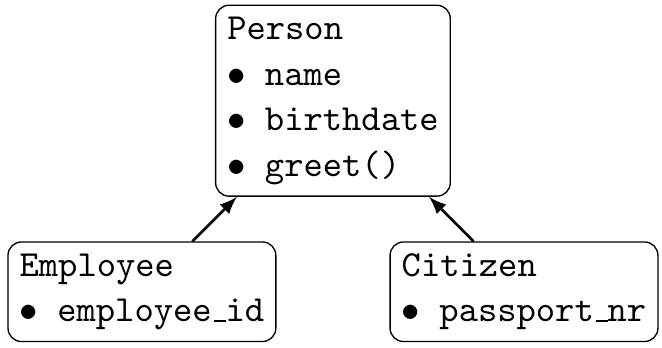
\includegraphics[width=\linewidth]{images/vererbung3.png}
    \end{center}
\end{minipage}\medskip
    
Polymorphism allows subclasses to define methods with the same name as those in the superclass, effectively overriding them. The specific method invoked depends on the actual object type at runtime, increasing interface flexibility.

\subsubsection{The \texttt{super()} Function}
The \texttt{super()} function provides access to methods and attributes of the superclass. It is primarily used within the subclass's \texttt{\_\_init\_\_} method to initialize inherited attributes, ensuring the proper setup of the base object state.

\begin{lstlisting}[language=Python]
class Person:
    def __init__(self, name):
        self.name = name

class Employee(Person):
    def __init__(self, name, employee_id):
        super().__init__(name) # Initialize superclass attributes
        self.employee_id = employee_id
\end{lstlisting}

\subsubsection{Abstract Classes}
Abstract classes serve as templates and cannot be instantiated directly. They define abstract methods that must be implemented by derived classes, enforcing a consistent interface. This requires the \texttt{abc} module.

\begin{lstlisting}[language=Python]
from abc import ABC, abstractmethod

class Vehicle(ABC):
    @abstractmethod
    def accelerate(self):
        pass

class Car(Vehicle):
    def accelerate(self):
        print('The car accelerates')
\end{lstlisting}

\subsection{Design Principles (SOLID)}
When constructing inheritance hierarchies, adhering to design principles ensures flexibility and maintainability:
\begin{itemize}
    \item \textbf{S}ingle Responsibility: A class should have only one responsibility and be responsible for exactly one thing.
    \item \textbf{O}pen-Closed: Classes should be open for extension (e.g., via inheritance) but closed for modification.
    \item \textbf{L}iskov Substitution: Objects of a superclass should be replaceable with objects of a subclass without affecting program correctness.
    \item \textbf{I}nterface Segregation: Clients should not be forced to depend on unused methods.
    \item \textbf{D}ependency Inversion: High-level modules should not depend on low-level modules; both should depend on abstractions.
\end{itemize}

\subsection{Aggregation and Composition}
Overusing inheritance can lead to a ``class explosion'' problem, significantly increasing 
complexity when combining multiple traits or options. 

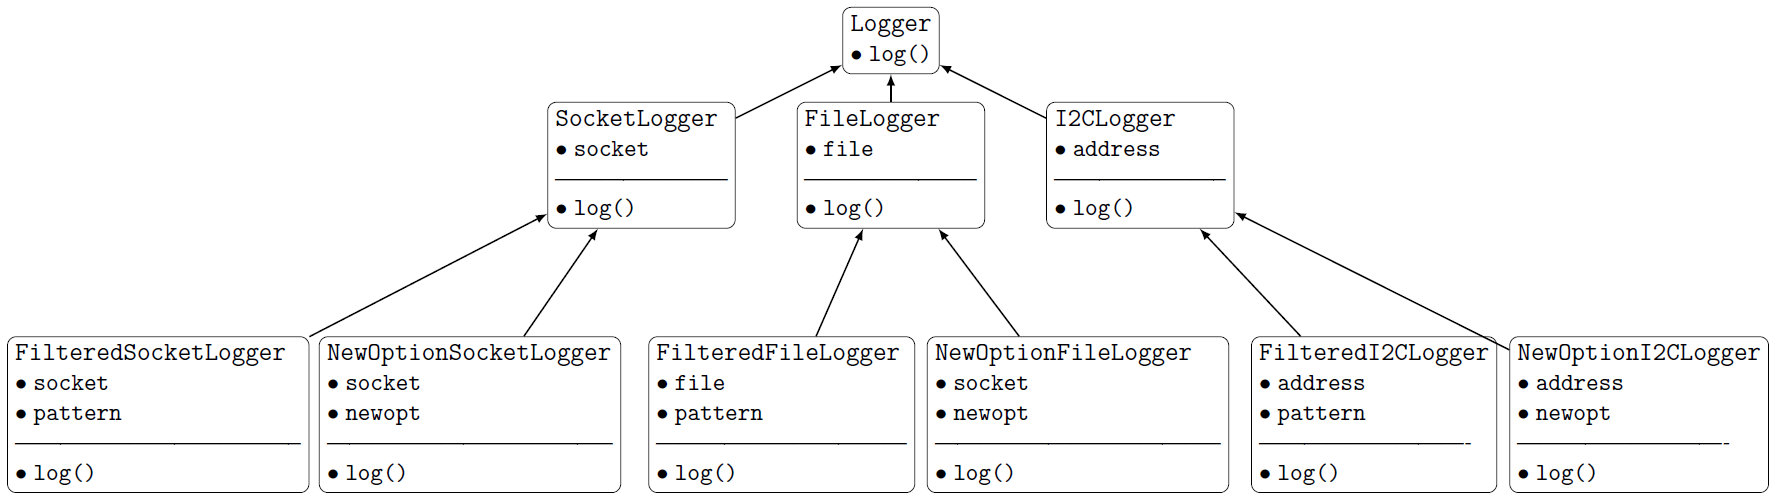
\includegraphics[width=\linewidth]{images/vererbung9.png}

Aggregation and composition offer 
structural alternatives by composing \textbf{classes based on dependencies rather than strict 
hierarchies.}\medskip

\begin{itemize}
    \item \textbf{Composition (is-a-part-of):} Implies a strong lifecycle dependency. The parent object owns and controls the lifetime of the contained objects. If the parent is destroyed, its parts are also destroyed (e.g., a Car and its Engine).
    \item \textbf{Aggregation (has-a):} Implies a loose lifecycle dependency. Contained objects can exist independently of the parent object and can be dynamically added or removed (e.g., a Library and its Books).
\end{itemize}

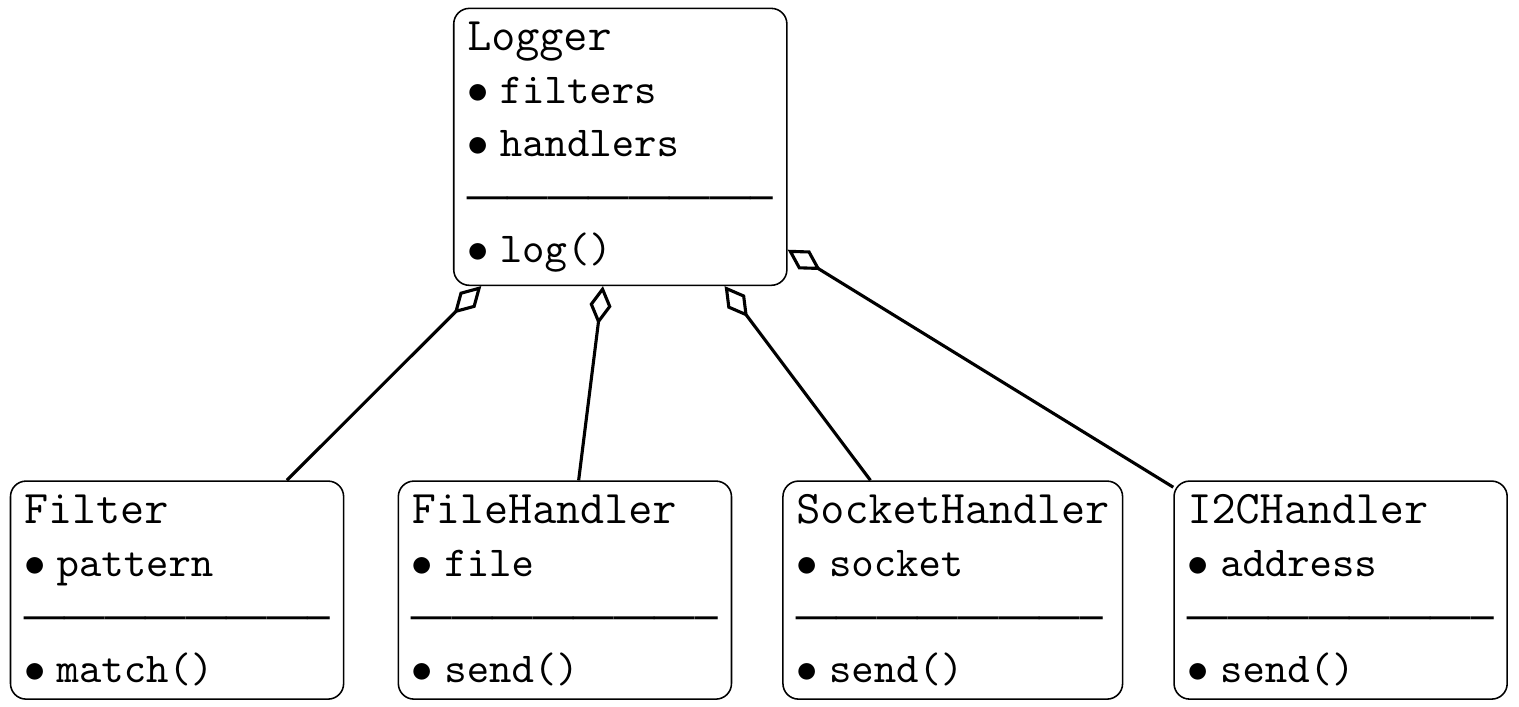
\includegraphics[width=\linewidth]{images/aggregation.png}

\lstinputlisting[language=Python]{code/aggregation.py}
        \section{NumPy}
\subsection{Introduction}
NumPy (Numerical Python) is a library for performing mathematical functions and operations on large multidimensional arrays. It provides:
\begin{itemize}
    \item \textbf{Speed}: Utilizes optimized C code, replacing slow standard Python \texttt{for} loops.
    \item \textbf{Vectorization}: Array-based operations are executed element-wise automatically.
    \item \textbf{Broadcasting}: Implicitly expands arrays of different shapes during arithmetic calculations.
\end{itemize}

\subsection{Creation of n-dimensional Arrays (\texttt{ndarray})}
The \texttt{ndarray} is a homogeneous data structure where each dimension is called an \textit{axis}.
\begin{itemize}
    \item \texttt{arr.ndim}: Number of dimensions.
    \item \texttt{arr.shape}: Tuple representing the size of each dimension. (rows, cols)
    \item \texttt{arr.dtype}: Data type of the array elements (e.g., \texttt{np.float64}, \texttt{np.int32}).
    \item \texttt{arr.astype(dtype)}: Returns a copy of the array cast to a specific type.
\end{itemize}

\subsubsection{Array Creation Methods}
\lstinputlisting[language=Python]{code/np_array_creation.py}


\resizebox{\columnwidth}{!}{
\begin{tabular}{l|l}
\textbf{Funktion} & \textbf{Resultat} \\ \hline
\texttt{np.ones((2,2))} & \texttt{array([[1., 1.], [1., 1.]])} \\
\texttt{np.ones\_like(arr1)} & \texttt{array([1, 1, 1])} \\
\texttt{np.zeros((2,2))} & \texttt{array([[0., 0.], [0., 0.]])} \\
\texttt{np.zeros\_like(arr1)} & \texttt{array([0, 0, 0])} \\
\texttt{np.full((2,2), 7.0)} & \texttt{array([[7., 7.], [7., 7.]])} \\
\texttt{np.full\_like(arr1, 7)} & \texttt{array([7, 7, 7])} \\
\texttt{np.eye(2)} & \texttt{array([[1., 0.], [0., 1.]])} \\
\texttt{np.linspace(0, 1, 5)} & \texttt{array([0., 0.25, 0.5, 0.75, 1.])} \\
\texttt{np.arange(0, 4, 0.5)} & \texttt{array([0, 0.5, 1, 1.5, 2, 2.5, 3, 3.5])} \\
\texttt{np.logspace(0, 1, 4)} & \texttt{array([1., 2.1544, 4.6416, 10.])} \\
\texttt{np.random.randn(3)} & \texttt{array([0.7576, 0.0135, -0.8934])} \\
\texttt{np.random.randint(0,10,3)} & \texttt{array([0, 5, 4])} \\
\end{tabular}}\medbreak

In \texttt{arange} è possibile inserire uno \texttt{step} negativo, per creare un array decrescente.

\crd{Attenzione al fatto che \texttt{end} è escluso dall'array,} se si vuole includere: (\texttt{end} $\pm$ \texttt{step})

\columnbreak

\subsection{Element Access}
\begin{itemize}
    \item \textbf{Indexing}: Axes are separated by commas within brackets (e.g., \texttt{arr[row, col]}).
    \item \textbf{Slicing}: Follows the \texttt{[start:end:step]} syntax across multiple
     axes. Slicing returns a \textbf{view}; modifications affect the original array. 
     Use \texttt{.copy()} to create an independent duplicate.
     \crd{END not included!}
    \item \textbf{Boolean Slicing}: Extracts subsets where a condition is \texttt{True} (e.g., \texttt{arr[arr > 5]}).
\end{itemize}


\textbf{Examples:}

\begin{center}
    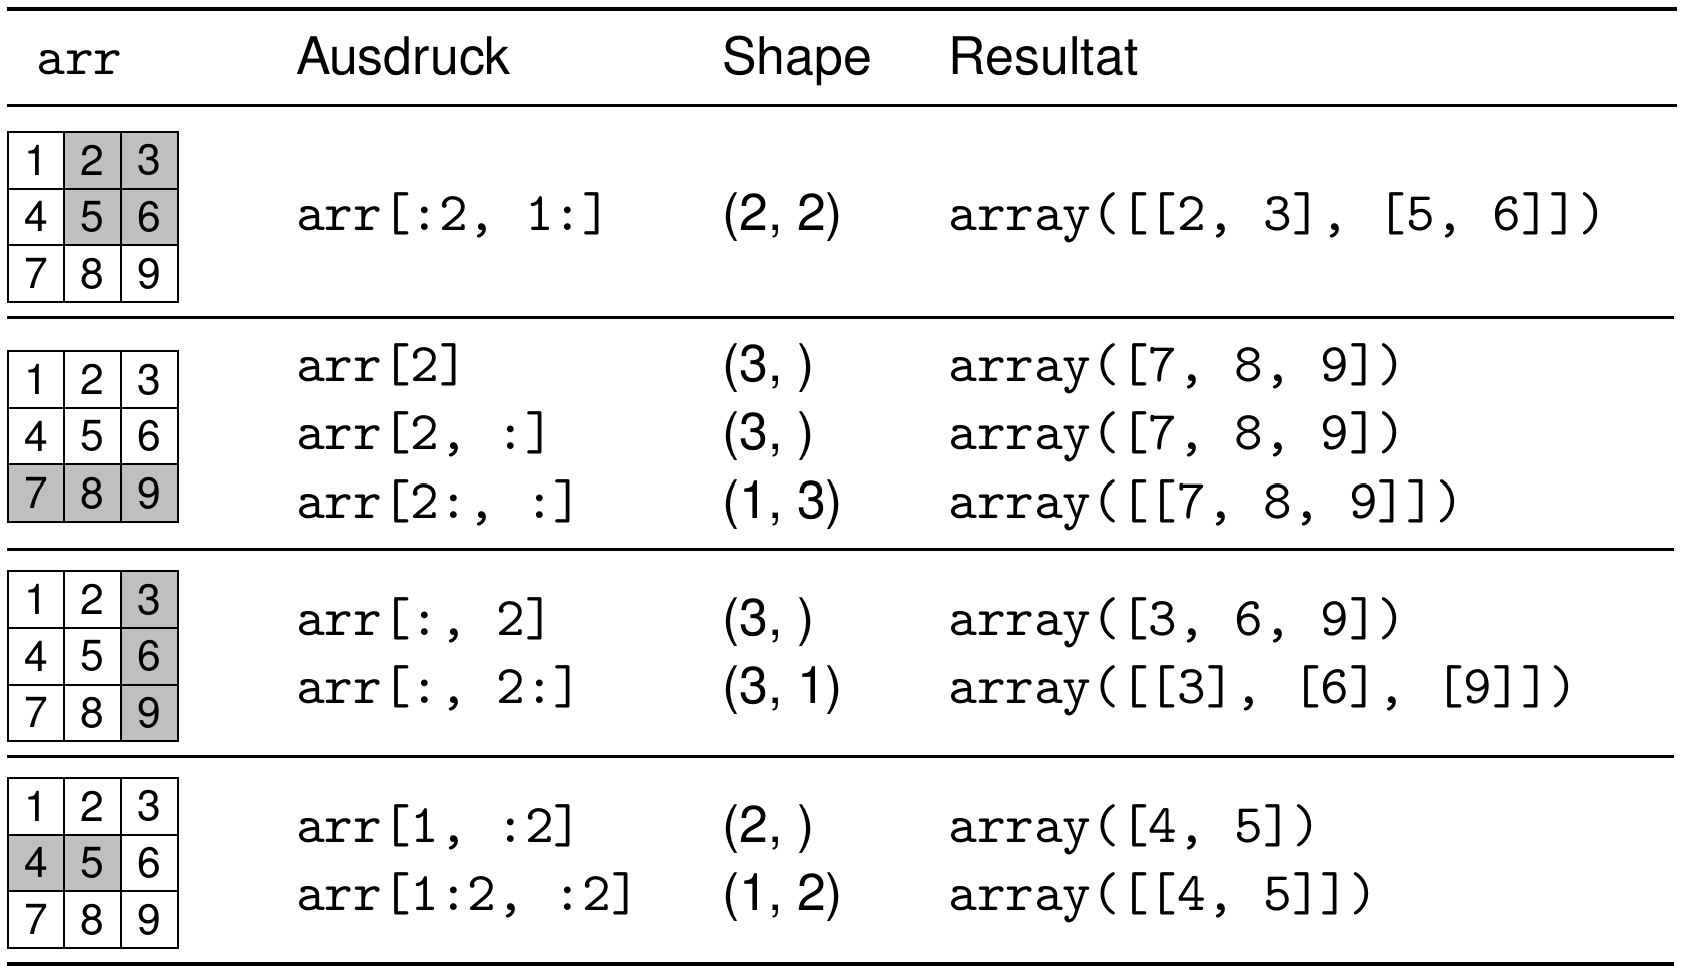
\includegraphics[width=0.7\linewidth]{images/slicing.png}
\end{center}

\begin{minipage}{0.45\columnwidth}
    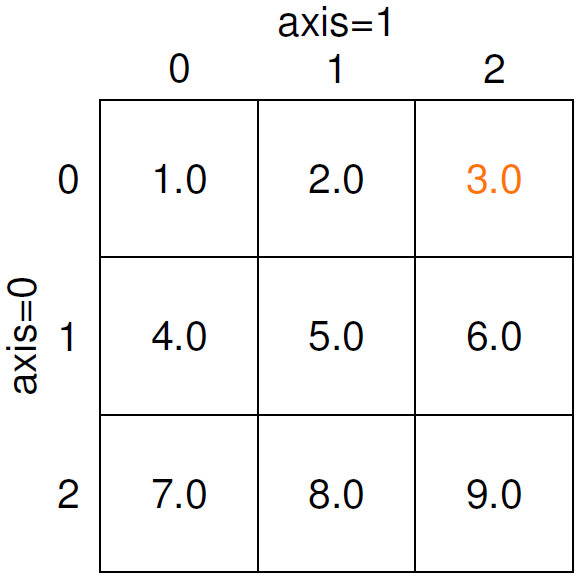
\includegraphics[width=\linewidth]{images/indizierung3.png}
\end{minipage}\hfill
\begin{minipage}{0.45\columnwidth}
    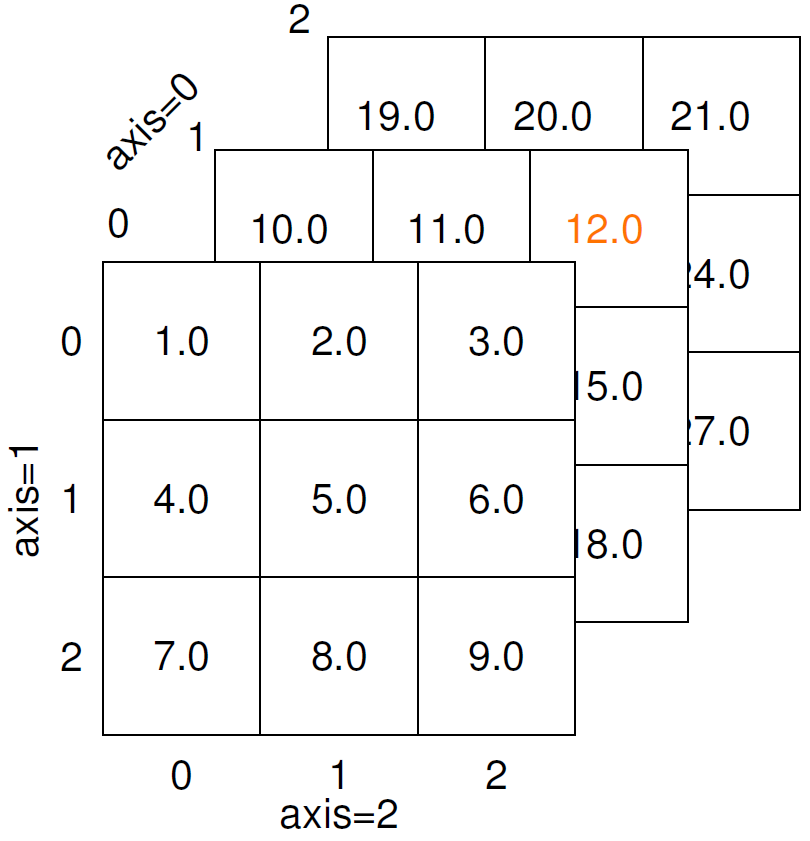
\includegraphics[width=\linewidth]{images/indizierung4.png}
\end{minipage}

The axes will always change when adding/removing dimesnions

\subsection{Broadcasting}
To perform operations on arrays of different shapes, NumPy automatically broadcasts the smaller array:
\begin{enumerate}
    \item Dimensions are inserted on the left until the number of dimensions (\texttt{ndim}) matches.
    \item Dimensions of size 1 are stretched to match the corresponding dimension of the other array.
    \item If sizes differ and neither is 1, a \texttt{ValueError} is raised.
\end{enumerate}

\subsection{Array Manipulation}
\subsubsection{Concatenation and Stacking}
\lstinputlisting[language=Python]{code/np_concatenation.py}


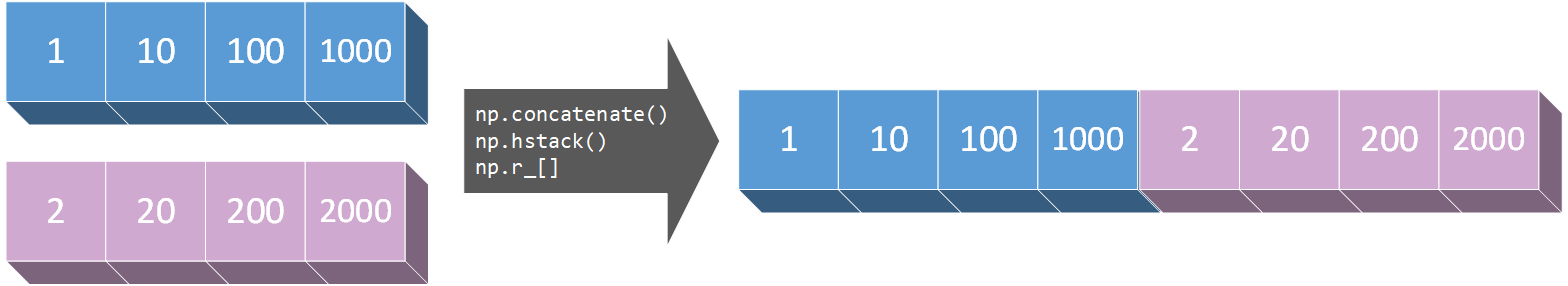
\includegraphics[width=\linewidth]{images/stacking_1D_1D.png}
\begin{center}
    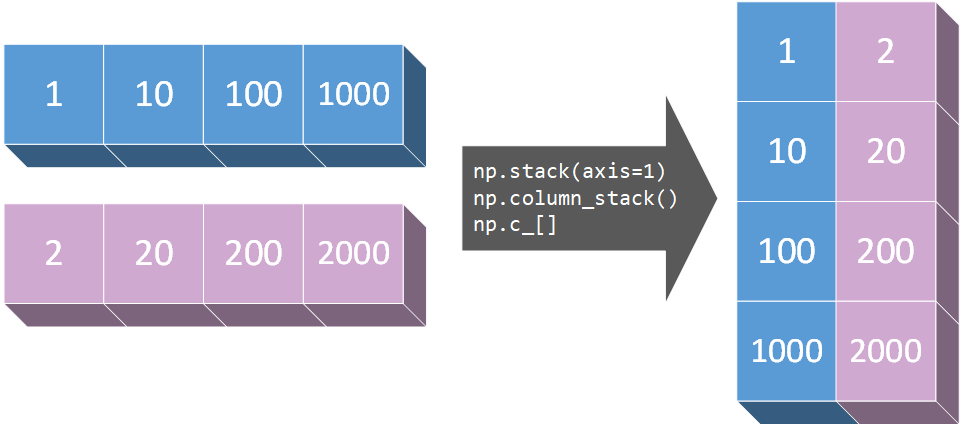
\includegraphics[width=0.7\linewidth]{images/stacking_1D_2D_spaltenweise.png}
\end{center}

\subsubsection{Dimension Changes}
\lstinputlisting[language=Python]{code/np_dimesnions.py}

Please note: arr.reshape(-1) only creates a view, not an actual copy


\subsection{Mathematical Functions}
NumPy provides vectorized universal functions (ufuncs) such as: \texttt{np.exp()}, \texttt{np.sin()}, \texttt{np.abs()}, \texttt{np.mean()}, \texttt{np.max()}, \texttt{np.std()}, and \texttt{np.cumsum()}.

% --- SUBSECTION: ADVANCED CONCATENATION & LINEAR ALGEBRA ---
\subsection{Concatenation}
\textbf{MATLAB-like Concatenation:}

\begin{itemize}
    \item \texttt{np.r\_}: Concatenates along the first axis (row-wise). It supports slice objects and individual values.
    \item \textit{Example:} \texttt{x = np.r\_[1:5, 15, 20:50:10]} $\rightarrow$ \texttt{[1, 2, 3, 4, 15, 20, 30, 40]}
    \item \texttt{np.c\_}: Concatenates along the second axis (column-wise). Ideal for creating column vectors.
    \item \textit{Example:} \texttt{y = np.c\_[0:3]} $\rightarrow$ \texttt{[[0], [1], [2]]}
\end{itemize}

\subsection{NumPy Linear Algebra: Multiplication Summary}

\subsubsection{Scalar and Vector Products}
\begin{itemize}
    \item \textbf{np.inner(a, b):} Best for the \textbf{Scalar Product} (inner product) of two vectors. 
    \begin{itemize}
        \item \textit{When to use:} Use it when you specifically want the inner product of vectors. It is clearer than \texttt{dot()} because it is restricted to this specific operation.
        \item \textit{Example:} \texttt{v1 = [1, 2]; v2 = [3, 4] $\to$ 1*3 + 2*4 = 11}.
    \end{itemize}
    
    \item \textbf{np.outer(a, b):} Computes the \textbf{Dyadic Product} (outer product).
    \begin{itemize}
        \item \textit{When to use:} Use it to create a matrix from two vectors (Column Vector $\times$ Row Vector).
        \item \textit{Example:} \texttt{v1 = [1, 2]; v2 = [3, 4] $\to$ [[3, 4], [6, 8]]}.
    \end{itemize}
\end{itemize}

\subsubsection{Matrix Multiplication: @ vs np.dot()}
While both perform standard matrix multiplication for 2D arrays, they behave differently for higher-dimensional tensors ($n > 2$).

\begin{itemize}
    \item \textbf{The @ Operator (np.matmul):} The standard for \textbf{Matrix Multiplication}.
    \begin{itemize}
        \item \textit{Behavior ($n > 2$):} It treats the array as a 'stack' of matrices and multiplies them across their final two dimensions.
        \item \textit{Recommendation:} This is the preferred method for standard matrix multiplication in modern Python (3.5+).
    \end{itemize}
    
    \item \textbf{np.dot(a, b):}
    \begin{itemize}
        \item \textit{Behavior ($n > 2$):} It calculates the sum of products across the \textbf{last} dimension of $a$ and the \textbf{penultimate} dimension of $b$.
        \item \textit{Result:} It effectively multiplies the first row of $a$ by EVERY column in each subsequent matrix of $b$, leading to a much larger resulting shape.
    \end{itemize}
\end{itemize}

\cor{Usually always use the \texttt{@} operator}
\subsubsection{Comparison Example ($n > 2$)}
\begin{lstlisting}[language=Python]
a = np.ones((2, 3, 3))
b = np.ones((2, 3, 3))

# Result: (2, 3, 3) -> Multiplies stacks independently
res_matmul = a @ b 

# Result: (2, 3, 2, 3) -> Multiplies every row by every column
res_dot = np.dot(a, b)     
\end{lstlisting}

        \newpage
        \section{Appendix}
\subsection{Type Conversion: \texttt{dict()} and \texttt{list()}}
\begin{itemize}
    \item \textbf{Tuple to Dict}: The \texttt{dict()} function can convert a list of 2-item tuples directly into key-value pairs.
    \item \textbf{Deduplication}: Since dictionary keys must be unique, converting a list of tuples to a \texttt{dict} automatically removes duplicate entries (keeping the last evaluated value for a given key).
    \item \textbf{Dict to List}: Converts the deduplicated dictionary back into a list of tuples using \texttt{list(dictionary.items())}.
\end{itemize}

\lstinputlisting[language=Python]{code/type_coversion.py}

\subsection{Decorators}
Decorators are functions that take another function as an argument to extend its behavior without modifying the original source code. They are denoted by the \texttt{@} symbol.

\begin{lstlisting}[language=Python]
def require_login(func):
    def wrapper(user):
        if user["logged_in"]:
            return func(user)
        print("Access denied.")
    return wrapper

@require_login
def view_dashboard(user):
    print(f"Welcome {user['name']}")
\end{lstlisting}


\subsection{Script Execution}
To distinguish between a script being run directly and a script being imported as a module, Python uses the \texttt{\_\_name\_\_} variable.

\begin{itemize}
    \item When run directly: \texttt{\_\_name\_\_ == "\_\_main\_\_"}.
    \item When imported: \texttt{\_\_name\_\_} equals the module's filename.
\end{itemize}

\begin{lstlisting}[language=Python]
def main():
    # Test code or entry point
    pass

if __name__ == "__main__":
    main()
\end{lstlisting}

\subsection{Distribuzioni Casuali in NumPy}

\begin{itemize}
    \item \textbf{np.random.rand}: Genera campioni da una distribuzione \textbf{uniforme} nell'intervallo $[0, 1)$. Ogni valore ha la stessa probabilità di essere estratto.
    \item \textbf{np.random.randn}: Genera campioni dalla distribuzione \textbf{normal standard} (Gaussiana) con media $\mu = 0$ e varianza $\sigma^2 = 1$.
\end{itemize}

\subsubsection{Trasformazione della Distribuzione Normale}
Per scalare e traslare la distribuzione normale standard $\mathcal{N}(0, 1)$ verso una distribuzione personalizzata $\mathcal{N}(\mu, \sigma^2)$, si applica la seguente formula lineare:

\[ X = \sigma \cdot \text{np.random.randn}(\dots) + \mu \]

Dove:
\begin{itemize}
    \item $\sigma$ (Sigma): Deviazione standard (controlla la "larghezza" della campana).
    \item $\mu$ (Mu): Media (sposta il centro della distribuzione).
\end{itemize}

\subsection{Indexing vs Slicing: Regola Rapida}

La differenza dipende dal tipo di selettore utilizzato per l'asse:

\begin{itemize}
    \item \textbf{Intero (Indexing)}: Se usi un numero secco (es. \texttt{arr[2]}), la dimensione viene \textbf{rimossa} (rank-1).
    \item \textbf{Range (Slicing)}: Se usi i due punti (es. \texttt{arr[2:3]}), la dimensione viene \textbf{mantenuta} (rank-2).
\end{itemize}

\subsubsection{Esempio Pratico}
Dato un array 2D di shape \texttt{(3, 3)}:
\begin{itemize}
    \item \texttt{arr[2, :]} $\rightarrow$ Risultato 1D, shape \texttt{(3,)}.
    \item \texttt{arr[2:3, :]} $\rightarrow$ Risultato 2D, shape \texttt{(1, 3)}.
\end{itemize}
    \end{layout}

    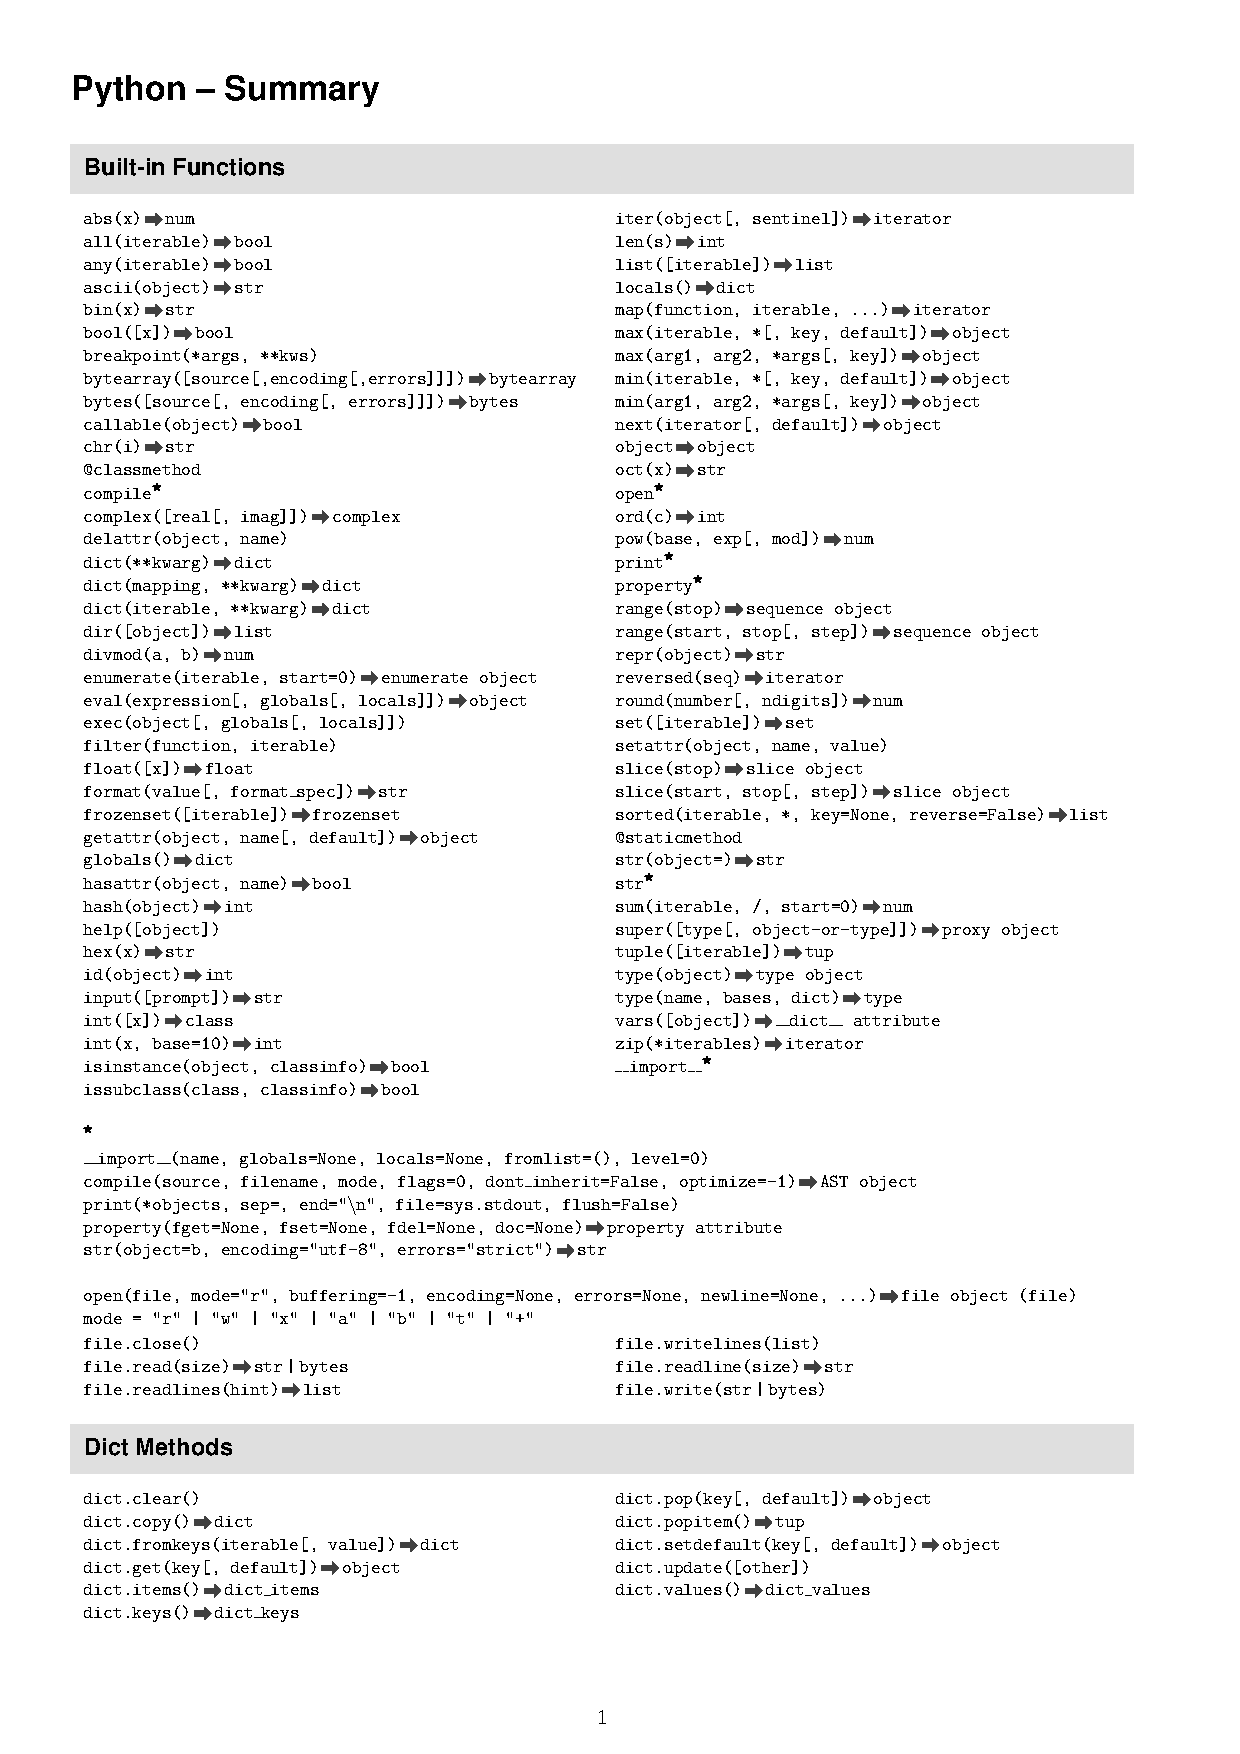
\includepdf[nup=2x1, pages=-]{Prog-ZF-py.pdf}
\end{document}